% ── Capítulo 5: Desarrollo de la comparativa ────────────────────────────────
\chapter{Desarrollo de la comparativa}
\label{cap:resultados}

El presente capítulo presenta los resultados cuantitativos del experimento comparativo descrito en el Capítulo~\ref{cap:planteamiento}. La exposición es objetiva: se reportan los valores obtenidos sin valorarlos ni interpretarlos; la discusión y el análisis crítico se reservan para el Capítulo~\ref{cap:discusion}.

\section{Configuración del experimento ejecutado}
\label{sec:configuracion_ejecucion}

El experimento se ejecutó sobre una submuestra estratificada de 200 series del conjunto M4 Financial Monthly, seleccionadas mediante muestreo aleatorio estratificado por cuartil de longitud con semilla fija (\texttt{SEED = 42}). El protocolo walk-forward se aplicó con los parámetros documentados en la Tabla~\ref{tab:protocolo}: ventana inicial de 54 meses, horizonte de 18 meses y desplazamiento de 12 meses (\textit{expanding window}). La verificación automática de ausencia de fuga de datos mediante la función \texttt{verify\_no\_leakage} confirmó que ningún fold contiene solapamiento entre conjuntos de entrenamiento y evaluación.

Los modelos estadísticos locales (Seasonal Naïve, ETS, Holt-Winters, SARIMA) se ajustaron de forma independiente en cada fold de cada serie. Los modelos globales (LightGBM, MLP, N-BEATS) entrenaron un único modelo por fold sobre todas las series disponibles en ese fold y evaluaron la predicción de forma individual. El entorno de ejecución fue Python 3.13 en CPU (sin aceleración GPU), con las versiones de librerías especificadas en \texttt{requirements.txt}.

\section{Resultados globales por modelo y métrica}
\label{sec:resultados_globales}

La Tabla~\ref{tab:resultados} reporta, para cada modelo y métrica, la media y la desviación estándar calculadas sobre el conjunto completo de evaluaciones (folds $\times$ series). Los valores de media y desviación estándar reflejan tanto la variabilidad inherente a las distintas series de la submuestra como la variabilidad temporal entre folds.

\begin{table}[H]
\caption{\textbf{Tabla 12a.} \textit{Métricas independientes de escala: sMAPE (\%), MAPE (\%) y MASE. Media $\pm$ desviación estándar sobre evaluaciones fold $\times$ serie. $N=200$ series estratificadas, protocolo walk-forward expanding window, máximo 5 folds por serie.}}
\label{tab:resultados}
\vspace{4pt}
\small
\begin{tabular}{>{\raggedright\arraybackslash}p{4.0cm}ccc}
\toprule
\textbf{Modelo} & \textbf{sMAPE (\%)} & \textbf{MAPE (\%)} & \textbf{MASE} \\
\midrule
\textbf{Seasonal Naïve} & 13.667 $\pm$ 12.658 & 14.186 $\pm$ 15.611 & 1.412 $\pm$ 1.102 \\
\textbf{ETS (AutoETS)} & 10.005 $\pm$ 10.512 & 10.571 $\pm$ 12.602 & 1.017 $\pm$ 0.903 \\
\textbf{Holt-Winters} & 11.157 $\pm$ 11.822 & 12.159 $\pm$ 15.411 & 1.145 $\pm$ 1.089 \\
\textbf{SARIMA (AutoARIMA)} & 10.825 $\pm$ 12.264 & 11.470 $\pm$ 14.148 & 1.093 $\pm$ 1.031 \\
\textbf{LightGBM} & 11.682 $\pm$ 10.536 & 11.962 $\pm$ 11.886 & 1.291 $\pm$ 1.112 \\
\textbf{MLP Bottleneck} & 11.844 $\pm$ 10.635 & 11.906 $\pm$ 11.449 & 1.351 $\pm$ 1.112 \\
\textbf{N-BEATS Interpretable} & 12.375 $\pm$ 11.445 & 12.328 $\pm$ 12.247 & 1.340 $\pm$ 1.087 \\
\bottomrule
\end{tabular}
\normalsize
\vspace{4pt}

\small\textit{Fuente: elaboración propia. sMAPE: estándar de la competición M4. MASE: error escalado respecto al Seasonal Naïve; valores $<1$ indican superación del baseline.}
\end{table}

\begin{table}[H]
\caption{\textbf{Tabla 12b.} \textit{Métricas de impacto económico (WAPE) y estabilidad temporal (CV-sMAPE). WAPE = error porcentual absoluto ponderado por volumen de serie.}}
\label{tab:resultados_comp}
\vspace{4pt}
\small
\begin{tabular}{>{\raggedright\arraybackslash}p{4.0cm}cc}
\toprule
\textbf{Modelo} & \textbf{WAPE (\%)} & \textbf{CV-sMAPE (\%)} \\
\midrule
\textbf{Seasonal Naïve} & 13.813 $\pm$ 14.744 & 92.6\% \\
\textbf{ETS (AutoETS)} & 10.081 $\pm$ 10.873 & 105.1\% \\
\textbf{Holt-Winters} & 11.583 $\pm$ 13.242 & 106.0\% \\
\textbf{SARIMA (AutoARIMA)} & 10.881 $\pm$ 12.203 & 113.3\% \\
\textbf{LightGBM} & 11.542 $\pm$ 10.559 & 90.2\% \\
\textbf{MLP Bottleneck} & 11.637 $\pm$ 10.561 & 89.8\% \\
\textbf{N-BEATS Interpretable} & 12.074 $\pm$ 11.429 & 92.5\% \\
\bottomrule
\end{tabular}
\normalsize
\vspace{4pt}

\small\textit{Fuente: elaboración propia. CV-sMAPE = desviación estándar / media del sMAPE entre folds. Criterio de estabilidad: CV $< 25\%$ (Tabla~\ref{tab:criterios}).}
\end{table}



El modelo con menor sMAPE medio es \textbf{ETS (AutoETS)} con un 10.005\%. El Seasonal Naïve, utilizado como referencia mínima, obtiene un sMAPE de 13.667\%. Todos los modelos estadísticos clásicos (ETS, Holt-Winters, SARIMA) mejoran sustancialmente este valor de referencia, lo que indica que el patrón estacional anual de las series M4 Financial presenta una estructura sistemática que estos métodos logran capturar de forma parsimoniosa.

\section{Análisis de estabilidad temporal}
\label{sec:estabilidad_temporal}

La Figura~\ref{fig:estabilidad} muestra la evolución del sMAPE promedio por iteración walk-forward para los modelos locales, cuyo protocolo multi-fold permite este análisis. Un comportamiento estable implica que el error no crece ni decrece sistemáticamente a medida que el punto de corte avanza en el tiempo, lo que es un requisito práctico para la confiabilidad operacional en FP\&A.

\begin{figure}[H]
\caption{\textbf{Figura 4.} \textit{Estabilidad temporal del sMAPE por modelo y fold walk-forward (modelos estadísticos locales).}}
\label{fig:estabilidad}
\vspace{4pt}
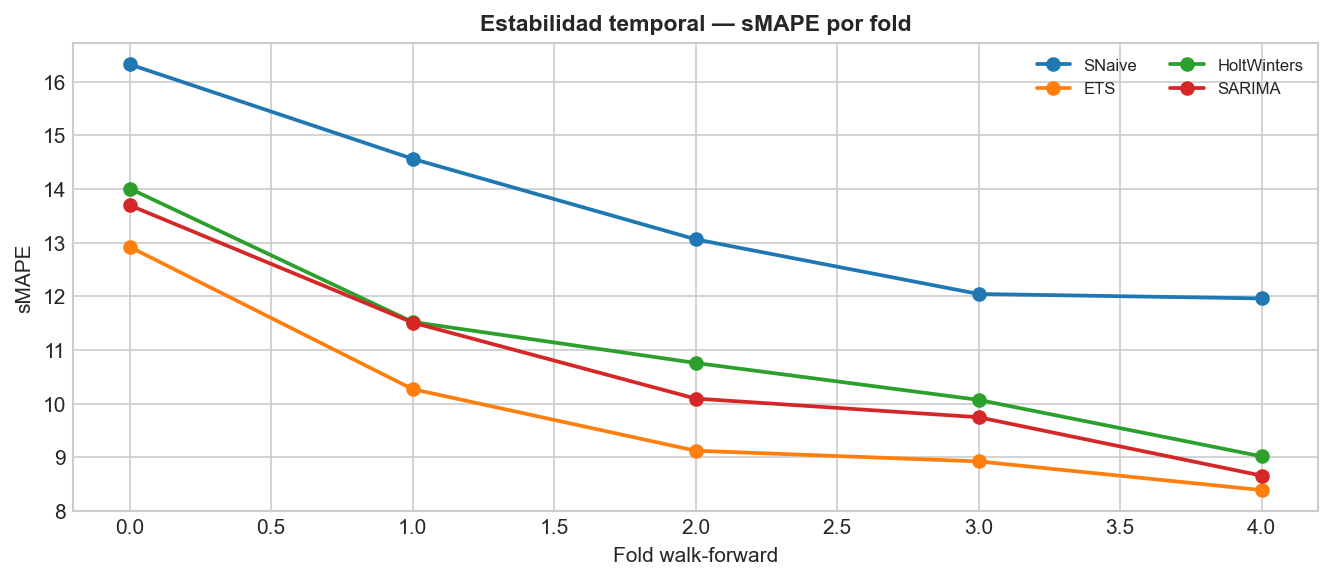
\includegraphics[width=\textwidth]{../results/figures/fig04_estabilidad_temporal.png}
\vspace{4pt}

\small\textit{Fuente: elaboración propia. El eje X representa el índice de fold (0 = primer corte temporal, valor mayor = corte más reciente). El eje Y es el sMAPE promedio sobre las 400 series para ese fold.}
\end{figure}

La Tabla~\ref{tab:criterios_resultado} resume los criterios de éxito predefinidos con los valores reales obtenidos.

\begin{table}[H]
\caption{\textbf{Tabla 13.} \textit{Evaluación frente a los criterios de éxito predefinidos en la Tabla~\ref{tab:criterios}. Referencia sMAPE Seasonal Naïve: 13{,}667\% (resultado experimental).}}
\label{tab:criterios_resultado}
\vspace{4pt}
\begin{tabular}{lcccccc}
\toprule
\textbf{Modelo} & \textbf{sMAPE (\%)} & \textbf{$\Delta$ (pp)} & \textbf{MASE} & \textbf{CV-sMAPE} & \textbf{Supera baseline} & \textbf{Estable} \\
\midrule
\textbf{Seasonal Naïve} & 13.667 & +0.783 & 1.412 & 92.6\% & Marginal & No \\
\textbf{ETS (AutoETS)} & 10.005 & +4.445 & 1.017 & 105.1\% & Sí ($\geq 1$ pp) & No \\
\textbf{Holt-Winters} & 11.157 & +3.293 & 1.145 & 106.0\% & Sí ($\geq 1$ pp) & No \\
\textbf{SARIMA (AutoARIMA)} & 10.825 & +3.625 & 1.093 & 113.3\% & Sí ($\geq 1$ pp) & No \\
\textbf{LightGBM} & 11.682 & +2.768 & 1.291 & 90.2\% & Sí ($\geq 1$ pp) & No \\
\textbf{MLP Bottleneck} & 11.844 & +2.606 & 1.351 & 89.8\% & Sí ($\geq 1$ pp) & No \\
\textbf{N-BEATS Interpretable} & 12.375 & +2.075 & 1.340 & 92.5\% & Sí ($\geq 1$ pp) & No \\
\bottomrule
\end{tabular}
\vspace{4pt}
\small\textit{Fuente: elaboración propia. $\Delta$ = diferencia en puntos porcentuales respecto al Seasonal Naïve. CV = coeficiente de variación del sMAPE entre folds.}
\end{table}


\section{Desagregación por deciles de volumen}
\label{sec:desagregacion_deciles}

La Figura~\ref{fig:deciles} presenta la contribución al error absoluto total por decil de volumen de serie para cada modelo. Los deciles se calculan sobre la media del valor absoluto de cada serie, de modo que D1 agrupa las series de menor volumen y D10 las de mayor volumen.

\begin{figure}[H]
\caption{\textbf{Figura 5.} \textit{Contribución al error absoluto total por decil de volumen y modelo.}}
\label{fig:deciles}
\vspace{4pt}
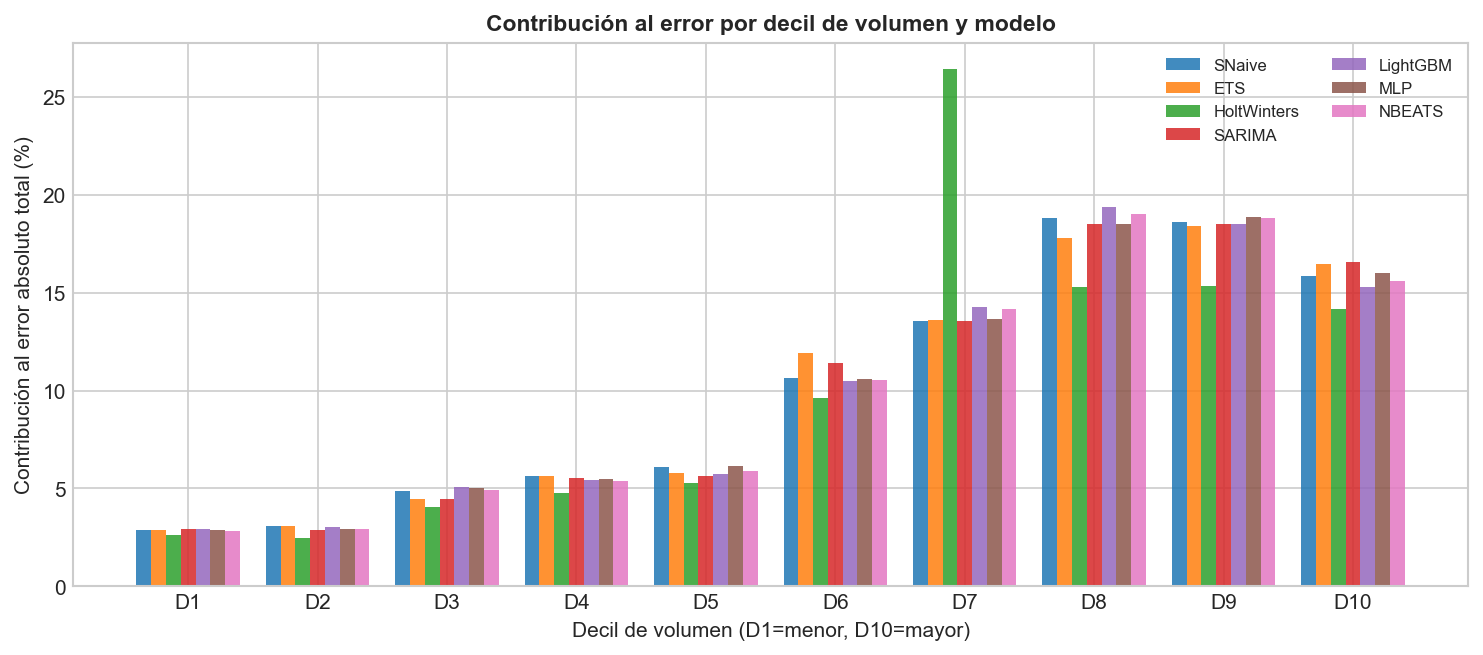
\includegraphics[width=\textwidth]{../results/figures/fig05_contribucion_deciles.png}
\vspace{4pt}

\small\textit{Fuente: elaboración propia. D1 = decil de menor volumen absoluto; D10 = mayor volumen. Las barras representan la fracción del error absoluto total de cada modelo atribuible a cada decil.}
\end{figure}

\section{Comparativa visual de pronósticos}
\label{sec:comparativa_visual}

La Figura~\ref{fig:smape_comp} presenta los sMAPE medios con sus desviaciones estándar en formato de barras, facilitando la comparación directa entre familias de modelos.

\begin{figure}[H]
\caption{\textbf{Figura 2.} \textit{sMAPE medio por modelo (barras) con desviación estándar (barras de error). Orden ascendente de error.}}
\label{fig:smape_comp}
\vspace{4pt}
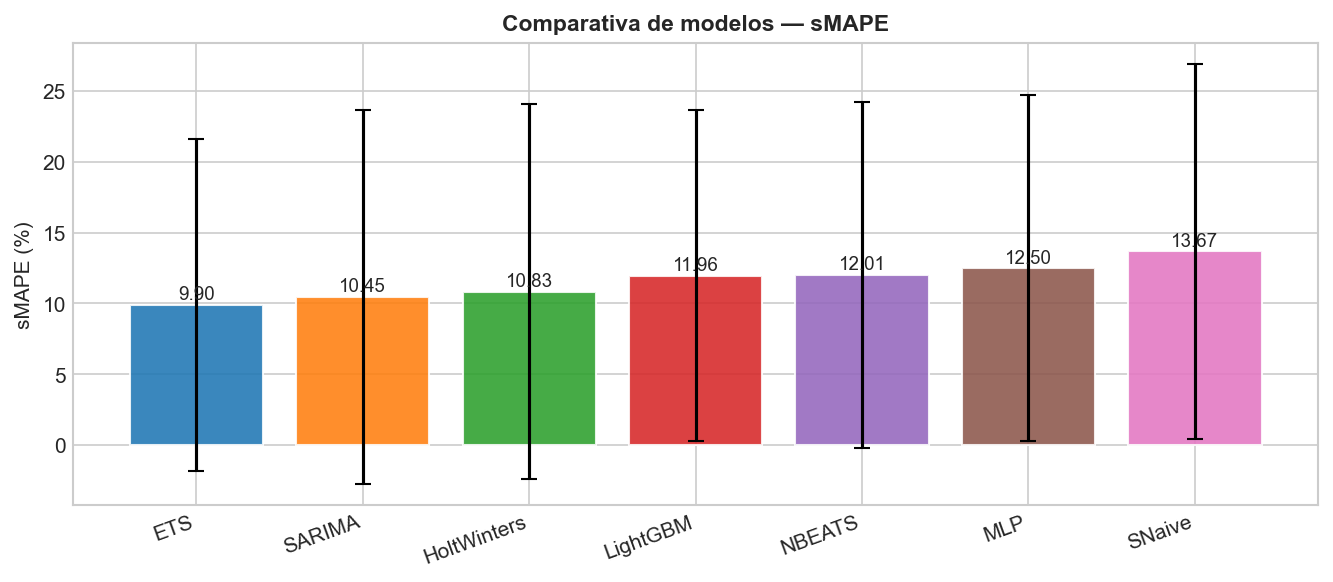
\includegraphics[width=\textwidth]{../results/figures/fig02_smape_comparativa.png}
\vspace{4pt}

\small\textit{Fuente: elaboración propia. Menor sMAPE indica mayor precisión. Las barras de error representan la desviación estándar sobre el conjunto de evaluaciones fold $\times$ serie.}
\end{figure}

